\documentclass[a4paper,10pt]{article}
\usepackage{hyperref}
%\usepackage[applemac]{inputenc}
\usepackage[french]{babel}
%\usepackage[latin1]{inputenc}
\usepackage{epsfig}
\usepackage{multirow}
\usepackage{amsmath}
\usepackage{amssymb}
\usepackage{comment}
\usepackage{epic}
\usepackage{color}

\usepackage{float}
\floatstyle{ruled}
\newfloat{Algorithm}{htp}{lop}

\setlength{\oddsidemargin}{0cm}
\setlength{\evensidemargin}{0cm}
\setlength{\marginparsep}{0cm}
\setlength{\marginparwidth}{0cm}
\setlength{\textwidth}{435pt}
\setlength{\textheight}{620pt}

\newcommand\fouriertransform[1]{\ensuremath{\mathcal{F}\left(#1\right)}}
\newcommand\inversefouriertransform[1]{\ensuremath{\mathcal{F}^{-1}\left(#1\right)}}
\newcommand\abs[1]{\ensuremath{\left|#1\right|}}
\newcommand\sign[1]{\ensuremath{\mathrm{sign}\left(#1\right)}}
\newcommand\sinc{{\ensuremath\mathrm{sinc}}}

\title{OBJET : Compression d'images façon JPEG}
\date{\today}
\author{}

\begin{document}
\maketitle

L'objectif de ce dernier travail sur machine est de construire une chaîne de compression et de décompression d'images, façon JPEG. Il ne s'agit pas d'implanter exactement l'algorithme de compression mais de travailler à plusieurs sur la réalisation d'une chaîne de compression et décompression d'images utilisant la plupart des principes de la compression JPEG. A l'instar du premier TP de MEDEV, vous devez vous organiser pour vous répartir le travail, mais cette fois, vous disposez de tous les outils nécessaires : gestion de version et partage de code, tests unitaires, etc...


\section{Introduction à la compression d'images façon JPEG}

La compression d'image JPEG\cite{JPEG} se fait à travers 4 étapes principales :
\begin{itemize}
\item une transformation dans un espace similaire à celui de Fourier (DCT)
\item une étape de quantification non conservatrice
\item une étape de \emph{codage en zig-zag}
\item une étape de stockage des données encodées suivant des algorithmes de compression sans perte
\end{itemize}

\begin{figure}[htbp]
\begin{center}
	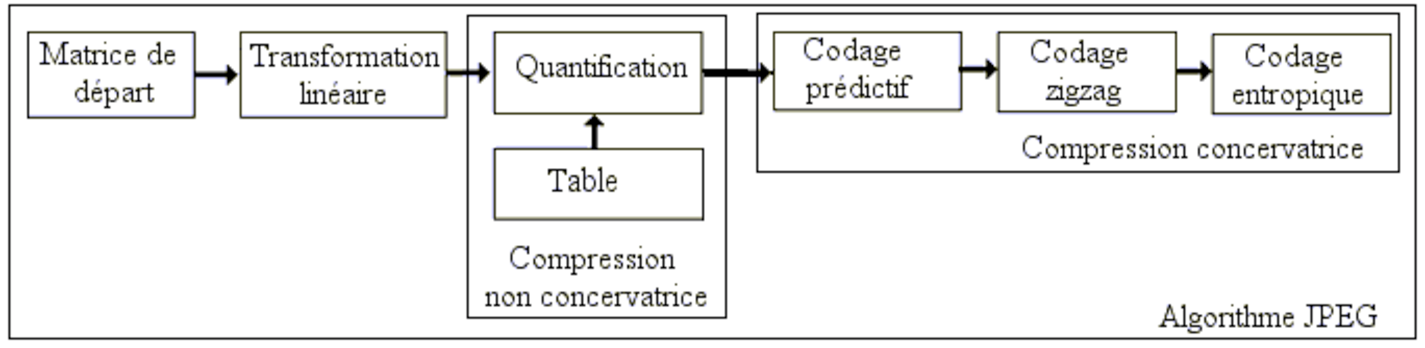
\includegraphics[width=\textwidth]{jpeg.pdf}
\caption{Principe de la compression JPEG}
\label{default}
\end{center}
\end{figure}

Inversement la décompression se fait de la façon suivante : 
\begin{itemize}
\item décompression des fichiers pour extraire les matrice quantifiées
\item déquantification
\item DCT inverse
\end{itemize}

\subsection{L'image}

A chaque pixel, caractérisé dans l'espace par ses coordonnées $( x , y )$, correspondent des intensités lumineuses sur trois couleurs primaires dites composantes R, V B pour rouge, vert et bleu. Ces nombres sont des entiers avec une valeur variant de 0 à 255. Il existe d'autres modèles de descriptions des couleurs ; la norme JPEG s'appuie sur le codage dit YIQ \cite{YIQ} (luminance, chrominance, saturation). Chacune des valeurs peut s'exprimer en fonction des composantes R, G, B. Par exemple, on a :
\begin{equation}
\left[ 
\begin{array}{c}
Y \\ I \\ Q \\
\end{array}
\right] =
\left( \begin{array}{ccc}
0.2999 & 0.587 & 0.114 \\
0.595716 & -0.24453 & -0.321263 \\
0.211456 & -0.522591 & 0.31135 \\
\end{array} \right)
\begin{array}{c}
R \\ G \\ B \\
\end{array}
\end{equation}


\subsection{Transformée discrète cosinus}

Les transformations linéaires agissent directement sur le signal et le transforment afin de révéler des caractéristiques propres à une compression efficace. Les transformations linéaires présentant ces qualités sont nombreuses mais la DCT, qui appartient à la famille des transformées de Fourier, présente un compromis nettement supérieur à ses concurrentes, ce qui lui a valu d'être retenue dans un grand nombre de normes dont la norme JPEG.

Prenons l'exemple d'une matrice de pixels représentant une image. Cette matrice est aussitôt divisée en blocs de 8x8 pixels. Il est alors possible de construire à l'aide de ces blocs un espace vectoriel muni d'opérations internes et externes. La transformation linéaire se fait donc sur ces blocs. Après transformation les blocs perdent leur nature initiale (ils ne représentent plus alors une image pour l'\oe il). Une transformation linéaire n'est donc que provisoire et suppose que son inverse soit effectuée avant restitution. Le problème soulevé est l'intérêt d'une telle transformation pour la compression. La DCT génère, quelles que soient les valeurs de l'image initiale, des valeurs transformées très différentes les unes des autres. Certaines sont devenues très grandes, d'autres très petites. Une annulation arbitraire de ces dernières n'entraîne ainsi qu'une distorsion réduite. La compression est alors le fruit d'un abandon d'un certain nombre de composantes. Il appartient au codeur en fonction de la distorsion maximale autorisée, ou bien en fonction du taux de compression demandé, de décider du nombre de composantes à abandonner.

On considère la matrice $P$ de taille $N$x$N$ (généralement $N$ vaut 8) définie par :
\begin{equation}
P_{ij} = c_j \sqrt{\frac{2}{N}} \cos{\left( \frac{(2i+1)j\pi}{2N}\right)}
\end{equation}

où les $c_j$ sont définis par : 
\begin{equation}
	c_0 = \frac{1}{\sqrt{2}}, c(j)=1 \quad 1 < j \leq N
\end{equation}

On remarque que $P^{-1} = P^{t}$. La transformée discrète cosinus d'un bloc $B$ est alors donnée par :
\begin{equation}
	F = P^{t} B P
\end{equation}

et la transformée inverse s'écrit alors : 
\begin{equation}
	B = P F P^{t} 
\end{equation}

\subsection{La quantification}

 La quantification représente la phase non conservatrice du processus de compression JPEG. Elle permet, moyennant une diminution de la précision de l'image, de réduire le nombre de bits nécessaires au stockage. Pour cela, elle réduit chaque valeur de la matrice DCT en la divisant par un nombre (quantum), fixé par une table (matrice 8 $\times$ 8) de quantification. Ce n'est ni plus ni moins qu'une division terme à terme de deux matrices.
 
Ultérieurement, lors de la restitution de l'image (décompression), il suffira de réaliser l'opération inverse (déquantification) en multipliant chaque valeur de la matrice quantifiée par le quantum correspondant, pour retrouver une matrice DCT déquantifiée, à partir de laquelle sera établie la matrice des pixels de sortie. La valeur du quantum peut être d'autant plus élevée que l'élément correspondant de la matrice DCT contribue peu à la qualité de l'image, donc qu'il se trouve éloigné du coin supérieur gauche.

Voici un exemple de matrice de quantification :

\begin{equation}
q_0 = \left(
\begin{array}{cccccccc}
3&5&7&9&11&13 & 15 &17 \\
5&7&9&11&13&15&17&19 \\
7&9&11&13&15&17&19&21\\
9&11&13&15&17&19&21&23\\
11&13&15&17&19&21&23&25\\
13&15&17&19&21&23&25&27\\
15&17&19&21&23&25&27&29\\
17&19&21&23&25&27&29&31\\
\end{array}
\right)
\end{equation}

L'étape finale du processus JPEG est le codage des images quantifiées qui réalise une compression conservatrice (sans perte). La phase de codage comporte en réalité trois phases, nous nous y intéresserons seulement partiellement.

\subsection{Codage}

Le codage de la matrice DCT quantifiée se fait en parcourant les éléments dans l'ordre imposé par une séquence particulière appelée séquence zigzag. On lit les valeurs en zigzags inclinés à $45^\circ$ en commençant par le coin supérieur gauche et en finissant en bas à droite. Cette séquence a la propriété de parcourir les éléments en commençant par les basses fréquences et de traiter les fréquences de plus en plus hautes. Puisque la matrice DCT contient beaucoup de composantes de hautes fréquences nulles, l'ordre de la séquence zigzag va engendrer de longues suites de 0 consécutives. Le résultat est une suite monodimensionnelle des coefficients quantifiés numérotés de 1 à 64. Ceci facilite de nouveau les étapes de compression suivantes : les codages RLC et VLC.

\begin{figure}[htbp]
\begin{center}
	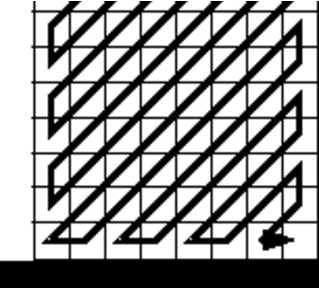
\includegraphics{zigzag.pdf}
\caption{Codage en zigzag}
\label{default}
\end{center}
\end{figure}

Deux mécanismes sont mis en \oe uvre pour comprimer la matrice DCT quantifiée :

D'une part les suites de valeurs nulles sont simplement codées en donnant le nombre de 0 successifs. C'est le codage RLC (Run Length Coding). Si une image contient une suite assez longue de pixels identiques, il devient intéressant de ne pas les recopier individuellement, mais plutôt de répertorier le couple nombre/valeur de couleur. On traite l'image ligne par ligne en recherchant les séquences de pixels de même valeur, en tirant profit des fortes corrélations horizontales. Le taux de compression obtenu est d'autant plus élevé que les zones de couleur uniforme sont grandes. Ce codage est sans perte.

D'autre part, les valeurs non nulles seront codées en utilisant une méthode de type statistique, comme le codage VLC (Variable Length Coding). Ce système est basé sur le fait que la probabilité d'apparition d'un élément codé sur N bits n'est pas la même pour tous les éléments. Par exemple, dans une image très sombre, la valeur 0 qui correspond au noir sera très fréquente. On a intérêt à coder sur un petit nombre de bits les valeurs qui sont les plus utilisées et à réserver des mots binaires de plus grande longueur aux valeurs les plus rares. Le codage VLC se combine remarquablement bien avec le codage RLC auquel il succède souvent, histoire d'augmenter encore le taux de compression. Dans la compression JPEG, on applique une compression RLC et un codage VLC, pour diminuer sans pertes la masse d'informations présentes. Un codage de Huffmann est un excellent exemple de codage VLC.

\subsection{Décompression}

La décompression consiste donc  à :
\begin{itemize}
\item ouvrir le fichier de données
\item rétablir la matrice DCT quantifiée en suivant le chemin inverse de la méthode Huffmann puis RLC
\item rétablir la matrice DCT déquantifiée en refaisant une simple multiplication terme à terme par la matrice de quantification
\item rétablir la matrice d'un bloc de pixels en effectuant la DCT inverse
\end{itemize}

\section{Travail demandé}

Il s'agit purement et simplement de vous répartir les tâches afin de réaliser une petite application de compression / décompression d'une image. Pour cela, vous veillerez à bien spécifier les classes et interfaces publiques afin de pouvoir vous répartir l'écriture du code. Chaque partie du code devra être testée individuellement (tests unitaires) avant l'intégration finale.

Vous pouvez utiliser OpenCV pour :
\begin{itemize}
	\item sa capacité à charger des images depuis un format non compressé (BMP par exemple)
	\item sa capacité à gérer des matrices
\end{itemize}

Vous ne pouvez évidemment pas utiliser OpenCV pour effectuer directement les différentes étapes de l'algorithme de compression / décompression.

La mise en \oe uvre du codage de Huffmann n'est pas obligatoire mais n'est  pas interdite non plus...
 
Les taux de compression respectifs des différents algorithmes utilisés seront vérifiés au passage.

Le rendu s'effectuera sous la forme d'un lien Github unique. il devra pointer vers un repository contenant le code source du logiciel, celui des tests unitaires et des éléments pour compiler tout cela (fichier CMakeLists.txt par exemple).


\begin{thebibliography}{9}
\bibitem{JPEG} JPEG, \emph{Wikipedia}, http://en.wikipedia.org/wiki/Jpeg
\bibitem{YIQ} YIQ,\emph{Wikipedia}, http://en.wikipedia.org/wiki/YIQ
\bibitem{chez} Compression d'images fixes : norme JPEG, http://www.chez.com/algorithmejpeg/dct.htm
\end{thebibliography}
\end{document}


